\vspace{12pt}
\section{Measurements of Film Thickness and Index of Refraction}
Spectrophotometry was used in order to determine the index of refraction of the films, their thickness, and the deposition rate during the PLD process. By recording the interference patterns of different wavelengths of light transmitted through the film on a high index of refraction substrate, the thickness is easily calculated with the formula \cite{Harrick1971},
 \begin{equation}
    2nd \cos(\phi) = \left(m+\frac{1}{2}\right) \lambda = \frac{\left(m+\frac{1}{2}\right)}{\nu}.
 \end{equation}

This well known formula is satisfied by the transmission maxima caused by constructive interference of light of wavelength $\lambda$ (or wavenumber $\nu = 1/\lambda$) at an angle of $\phi$ within a film of thickness $d$ and index of refraction $n$. If the order of the fringe is not known and the transmitted angle within the material is not known but the incident angle $\theta$ is, then any two fridges can be used by combining the above equation with Snell's law and letting $\Delta m$ be the number of peaks between the two maxima. This gives
 \begin{equation}
     d = \frac{\Delta m}{2 \Delta \nu_{if} \sqrt{n^2-\sin^2{\theta}}}.
     \label{eq:film:thickness}
 \end{equation}
If the index of refraction is not known, then by recording the interference pattern at different incident angles, the index of refraction can be measured by combining the above constructive interference equation with Snell's Law for relating the incident angle $\theta$ to the transmitted angle $\phi$, yielding 
 \begin{equation}
     n = \sqrt{\frac{\sin^2{\theta_1}\Delta\nu_1^2-\sin^2{\theta_2}\Delta\nu_2^2}{\Delta\nu_1^2-\Delta\nu_2^2}}.
     \label{eq:film:index}
 \end{equation}
Multiple adjacent fringes can be combined, improving the accuracy of this method provided the index of refraction is relatively constant over that range. But, by measuring the distance between several adjacent fringes, a determination of the change in index of refraction can be made. Using this method with different incident angles provides a baseline for film thickness determination, from which the deposition rate can be found. 

\begin{figure}
    \centering
    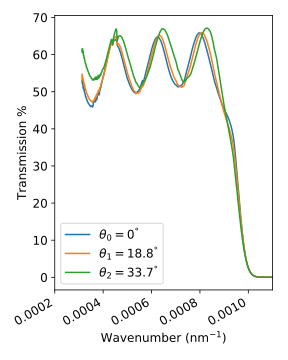
\includegraphics{Figures/190515-spectrophotometry.pdf}
    \caption{Transmission data as a function of wavenumber $\nu$. The peak locations can be modelled with a sine curve and extracted in order to obtain $\Delta \nu$ for a given incident angle $\theta$. Film was deposited on silicon with 20,000 pulses from a target made by combustion spray pyrolysis.}
    \label{fig:film:sp:transmVsAngle}
\end{figure}

To determine peak location, two different fitting methods were employed. Peak maxima or minima were determined by plotting the derivative of transmission vs wavenumber and solving for zero. Additionally, since the transmission as a function of wavenumber is expected to be a sine function, a sine curve was fit to the data, and the positions of either minima or maxima were found and then used in the determination of the index of refraction. 

In the data set shown in Figure \ref{fig:film:sp:transmVsAngle}, the two most separate maxima ($m=2$), at an incident angle of $\theta_0 = 0$\textdegree, are separated by $\Delta \nu_0 = 0.0003501 $ nm$^{-1}$, while for an incident angle of $\theta_1 = 18.8$\textdegree\ the separation is $\Delta \nu_1 = .00035643$ nm$^{-1}$. This provides a value for index of refraction $n = 1.72$. Repeating this procedure with the third incident angle and averaging gives an index of refraction of $n=1.75$. Using this $n$, now with equation \ref{eq:film:thickness} give a thickness of 1600 nm. Since this value of $n$ was obtained from a sample made at a laser energy density of 2.8 J/cm$^2$ with 20,000 pulses, the deposition rate at that energy density is 0.8 \AA/pulse. 

As a point of comparison, this method was used on a film grown from 8,000 pulses at 2.3 J/cm$^2$ and using $n=1.75$ was found to be 430 nm, a growth rate of 0.5 \AA/pulse. This thickness is near the lower limit of the spectrophotometer's range to measure the thickness for thin films on silicon. Applying this growth rate to a film made with the same energy density, but with 6,000 pulses, gives an estimated thickness of 320 nm. Cleaving this sample and examining it edgewise in the scanning electron microscope provides an alternative method of measurement as seen in Figure \ref{fig:film:sem:thickness}, which is $\sim 400$ nm. Given the uncertainties in both the SEM thickness calculation and the determination of the index of refraction from a limited set of interference patterns, this is a reasonable estimate of thickness and one applied to the conversion to conductivity from the impedance measurements. These values for growth rate may introduce a source of systematic error on the conductivity measurements. Improvements to this method should include growing films in a wider range of thicknesses. In addition, rather than measuring the transmission of light, measuring the reflection of light would allow a wider range of substrate materials and the absorbance of the substrate would not limit the range of wavelengths available for these calculations.

\begin{figure}
    \centering
    \includegraphics[width=.7\linewidth]{Figures/BZG-XS10-Si_20000x_BSE_014.pdf}
    \caption{Scanning electron microscopy of Gd:BaZrO\textsubscript{3} film deposited on silicon with 6,000 laser pulses. Target was produced by solid state reaction.}
    \label{fig:film:sem:thickness}
\end{figure}